\sisetup{separate-uncertainty=true}

\begin{frame}{Event Analysis}
  \begin{itemize}
    \item Calculation of measurable muon rate
    \begin{itemize}
      \item Considering detector geometry, \\
      expected muon rate and angular distribution
    \end{itemize}
    \item Distinguish events by the number of traversed detector layers (planes)
    \begin{itemize}
      \item  Event with n traversed planes: n-plane-event (npE)
    \end{itemize}
  \end{itemize}
  \begin{center}
  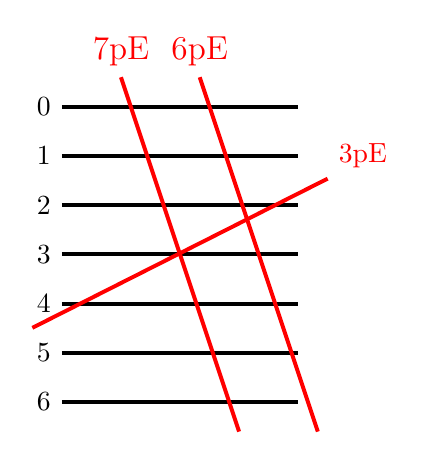
\begin{tikzpicture}[scale=0.5]

    \draw[black, line width = 0.5mm] (-3,0) node[left] {6} -- (3,0);
    \draw[black, line width = 0.5mm] (-3,1.25) node[left] {5} -- (3,1.25);
    \draw[black, line width = 0.5mm] (-3,2.5) node[left] {4}-- (3,2.5);
    \draw[black, line width = 0.5mm] (-3,3.75) node[left] {3} -- (3,3.75);
    \draw[black, line width = 0.5mm] (-3,5) node[left] {2} -- (3,5);
    \draw[black, line width = 0.5mm] (-3,6.25) node[left] {1} -- (3,6.25);
    \draw[black, line width = 0.5mm] (-3,7.5) node[left] {0} -- (3,7.5);

    \draw[red, line width = 0.5mm] (-1.5,8.25) node[above] {\large 7pE} -- (1.5,-0.75);
    \draw[red, line width = 0.5mm] (0.5,8.25) node[above] {\large 6pE} -- (3.5,-0.75);
    \draw[red, line width = 0.5mm] (3.75,5.675) node[above right]{3pE} -- (-3.75,1.885);

  \end{tikzpicture}
  \end{center}
\end{frame}
\begin{frame}{Event Analysis}
  \begin{itemize}
    \item Comparison of evaluated data to expectation
  \end{itemize}
  \begin{figure}[H]
    \centering
    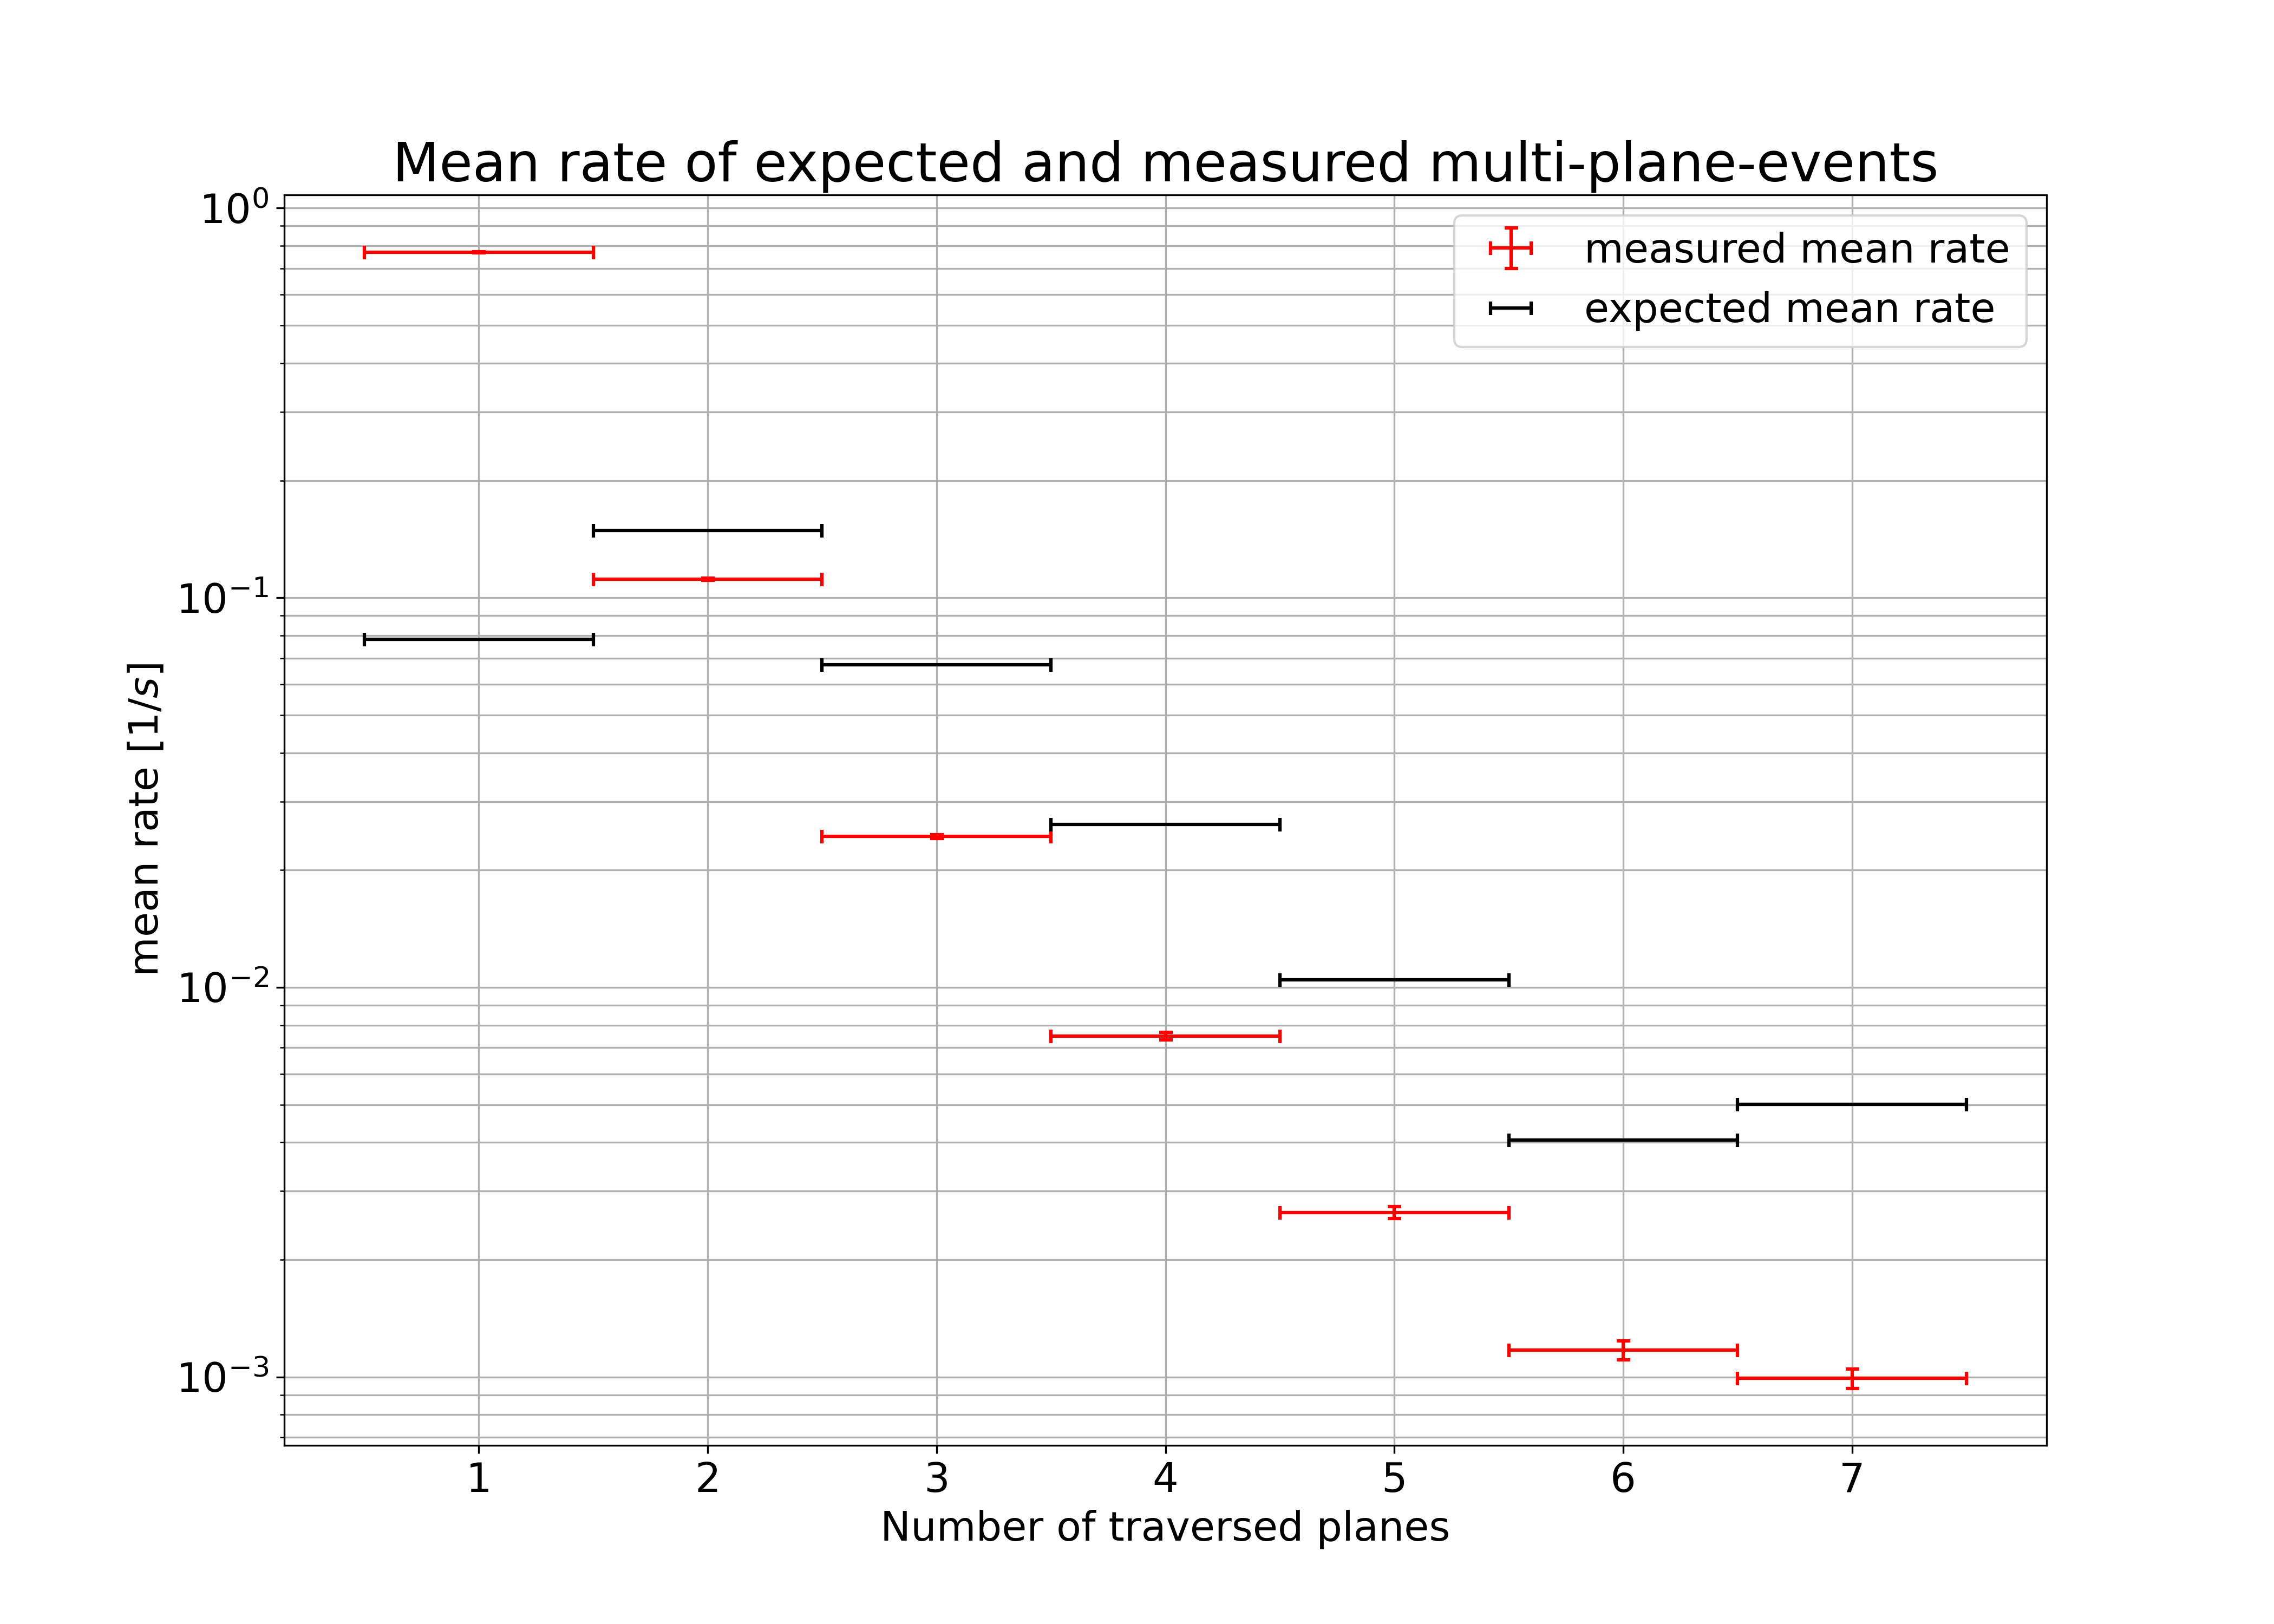
\includegraphics[width=.8\textwidth]{rate_comparison}
    %\caption{Comparison of estimated and measured muon rate}
  \end{figure}
  \begin{itemize}
	\item What are the reasons for the overestimation?
  \end{itemize}
\end{frame}

\begin{frame}{Event Analysis}
  \begin{itemize}
    \item Differences in measured mean hit rate per plane
    \item Dependency on thresholds
  \end{itemize}
  \begin{figure}[H]
    \centering
    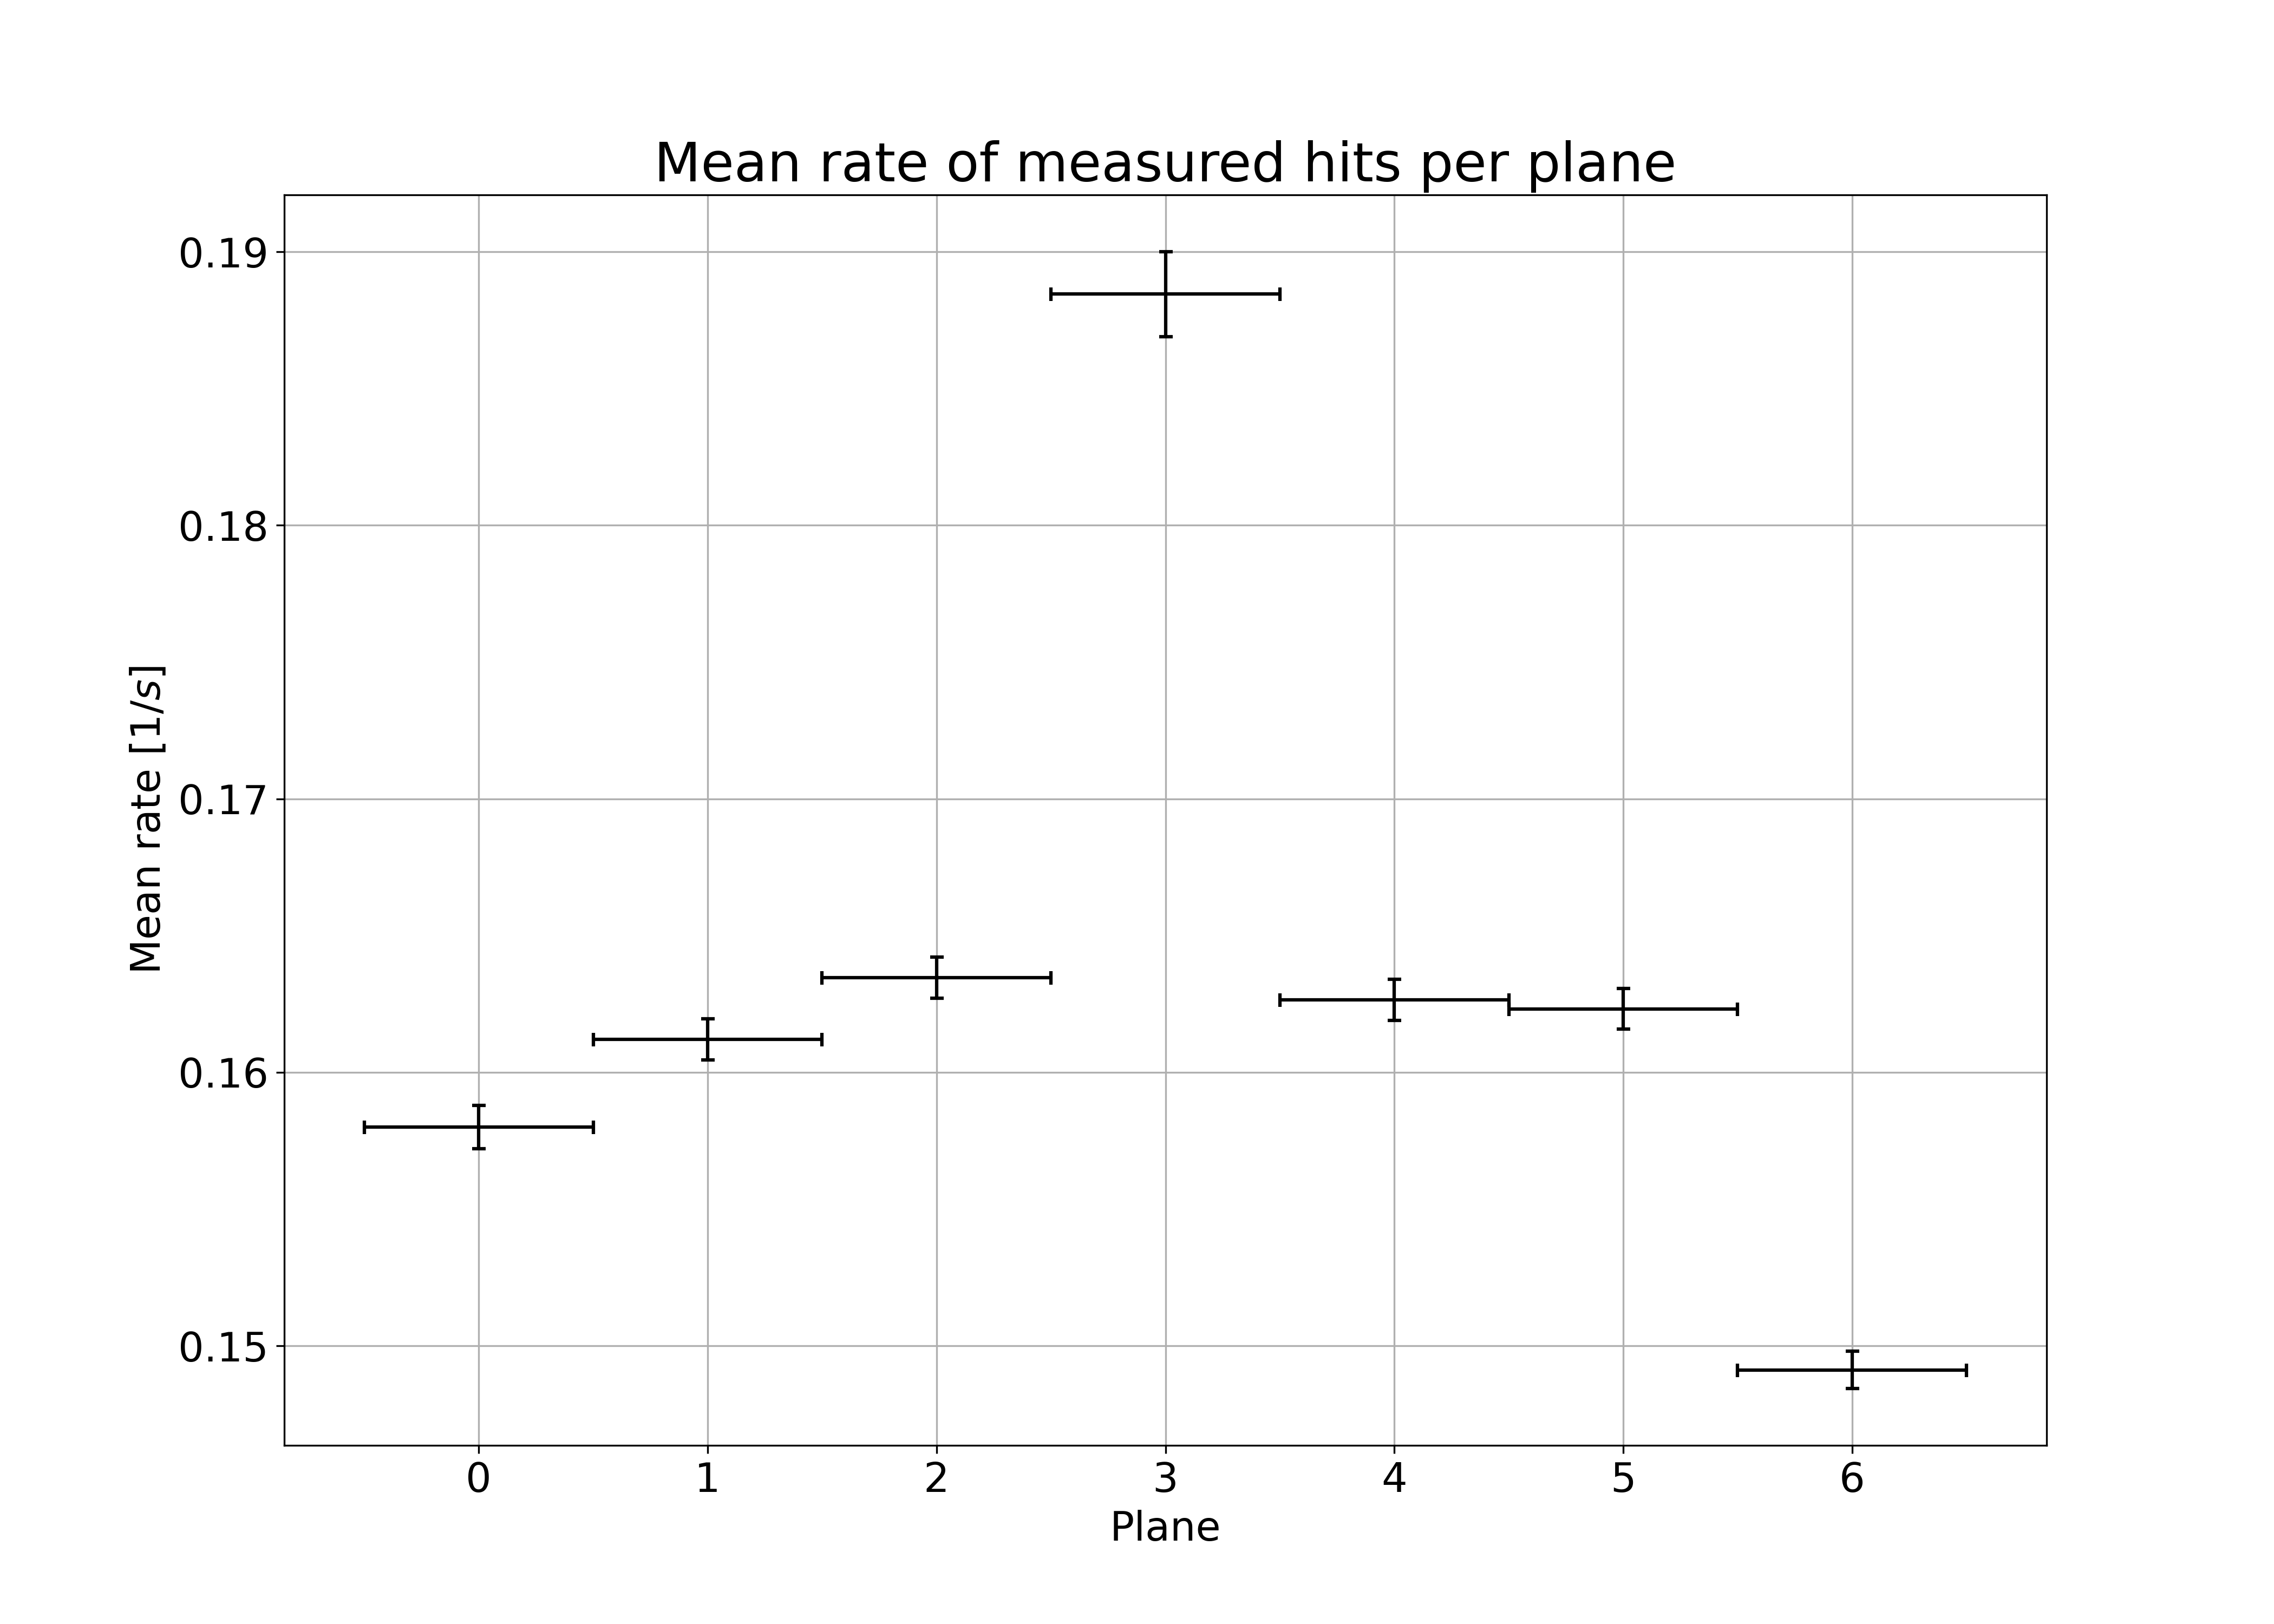
\includegraphics[width=.65\textwidth]{rate_per_plane}
    %\caption{Mean rate of measured hits}
  \end{figure}
  \begin{center}
  \resizebox{0.8\textwidth}{!}{%
  	\sisetup{table-figures-uncertainty=2,
  		table-figures-decimal=1,
  		table-number-alignment = center,
  		table-text-alignment = center}
  	%\centering
  	\begin{tabular}{cccccccc}
  		\toprule
  		Plane & 0 & 1 & 2 & 3 & 4 & 5 & 6 \\
  		\midrule
  		Threshold $[DAC]$ & 27.2(6) & 31.3(6) & 22.8(4) & 12.7(5) & 21.4(5) & 16.1(6) & 20.2(6) \\
  		\bottomrule
  	\end{tabular}
    %\caption{Thresholds of each plane}
  } % end of scope of "\resizebox"  directive
  \end{center}
\end{frame}

\begin{frame}{Event Analysis}
  \begin{itemize}
    \item Check for events with hits on not consecutive planes
    \begin{itemize}
      \item (i.e. planes 1,2,3,4,5,7 registering a hit lead to false 6pE)
    \end{itemize}
    \item Corrected mean rate by removing not consecutive plane events
    \item Further analysis with track information
  \end{itemize}
  \begin{figure}[H]
    \centering
    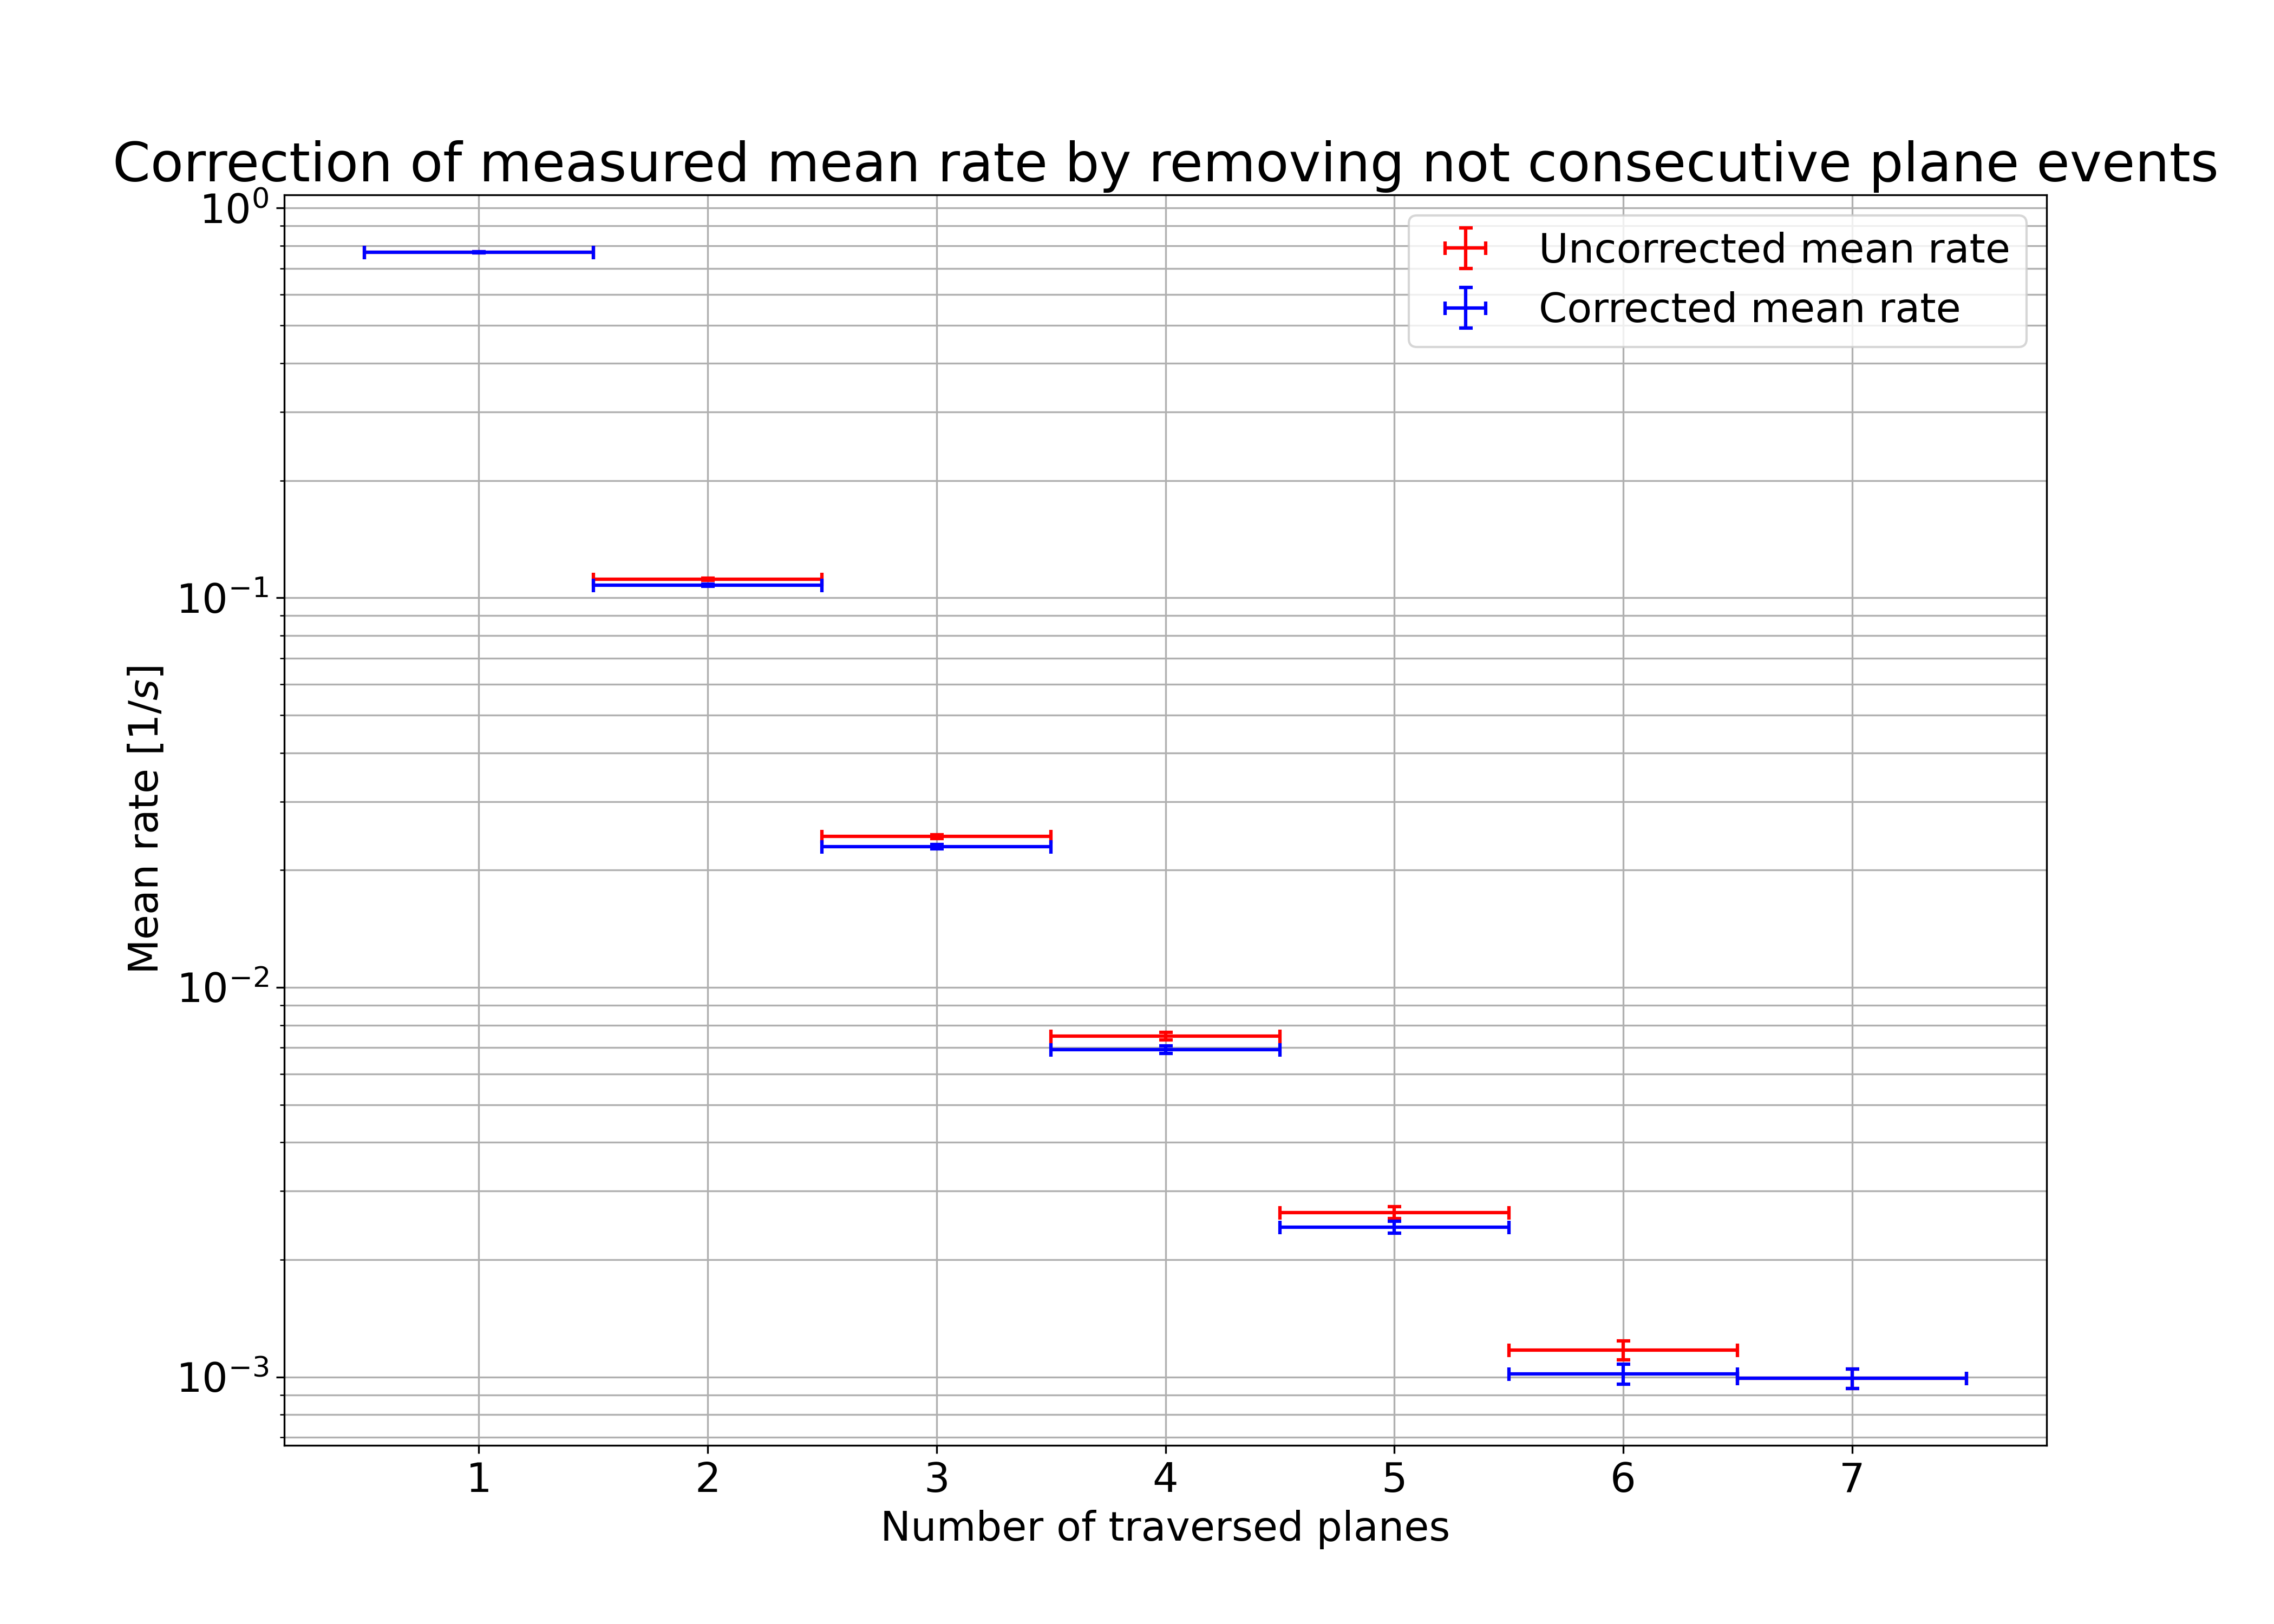
\includegraphics[width=.6\textwidth]{rate_correction}
    \caption{Mean rate correction by not consecutive plane events}
  \end{figure}
\end{frame}

\begin{frame}{Track Analysis}
  \begin{itemize}
    \item Track visualized with 2-dimensional projection
    \item Alignment with data of testbeam June 2020
    \item Possibility to classify events as valid or fake track
  \end{itemize}
  \begin{figure}[H]
    \centering
    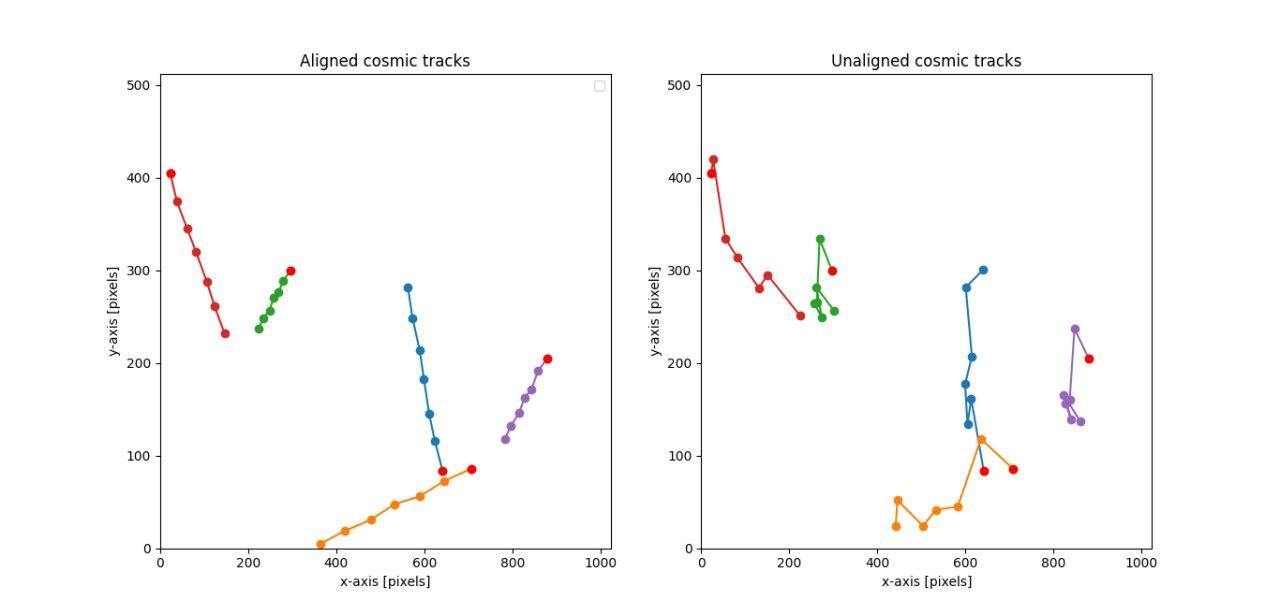
\includegraphics[width=.8\textwidth]{track_visual}
    \caption{Alignment with 2020 testbeam data}
  \end{figure}
\end{frame}

\begin{frame}{Track Analysis}
  \begin{itemize}
    \item Linear fit on 2D-track projections
    \item Analysis of $\chi^2_{red}$-distribution and angular distribution
    \item Open questions regarding the angular distribution (e.g. too few entries at small angles)

  \end{itemize}
  \begin{figure}[H]
    \centering
    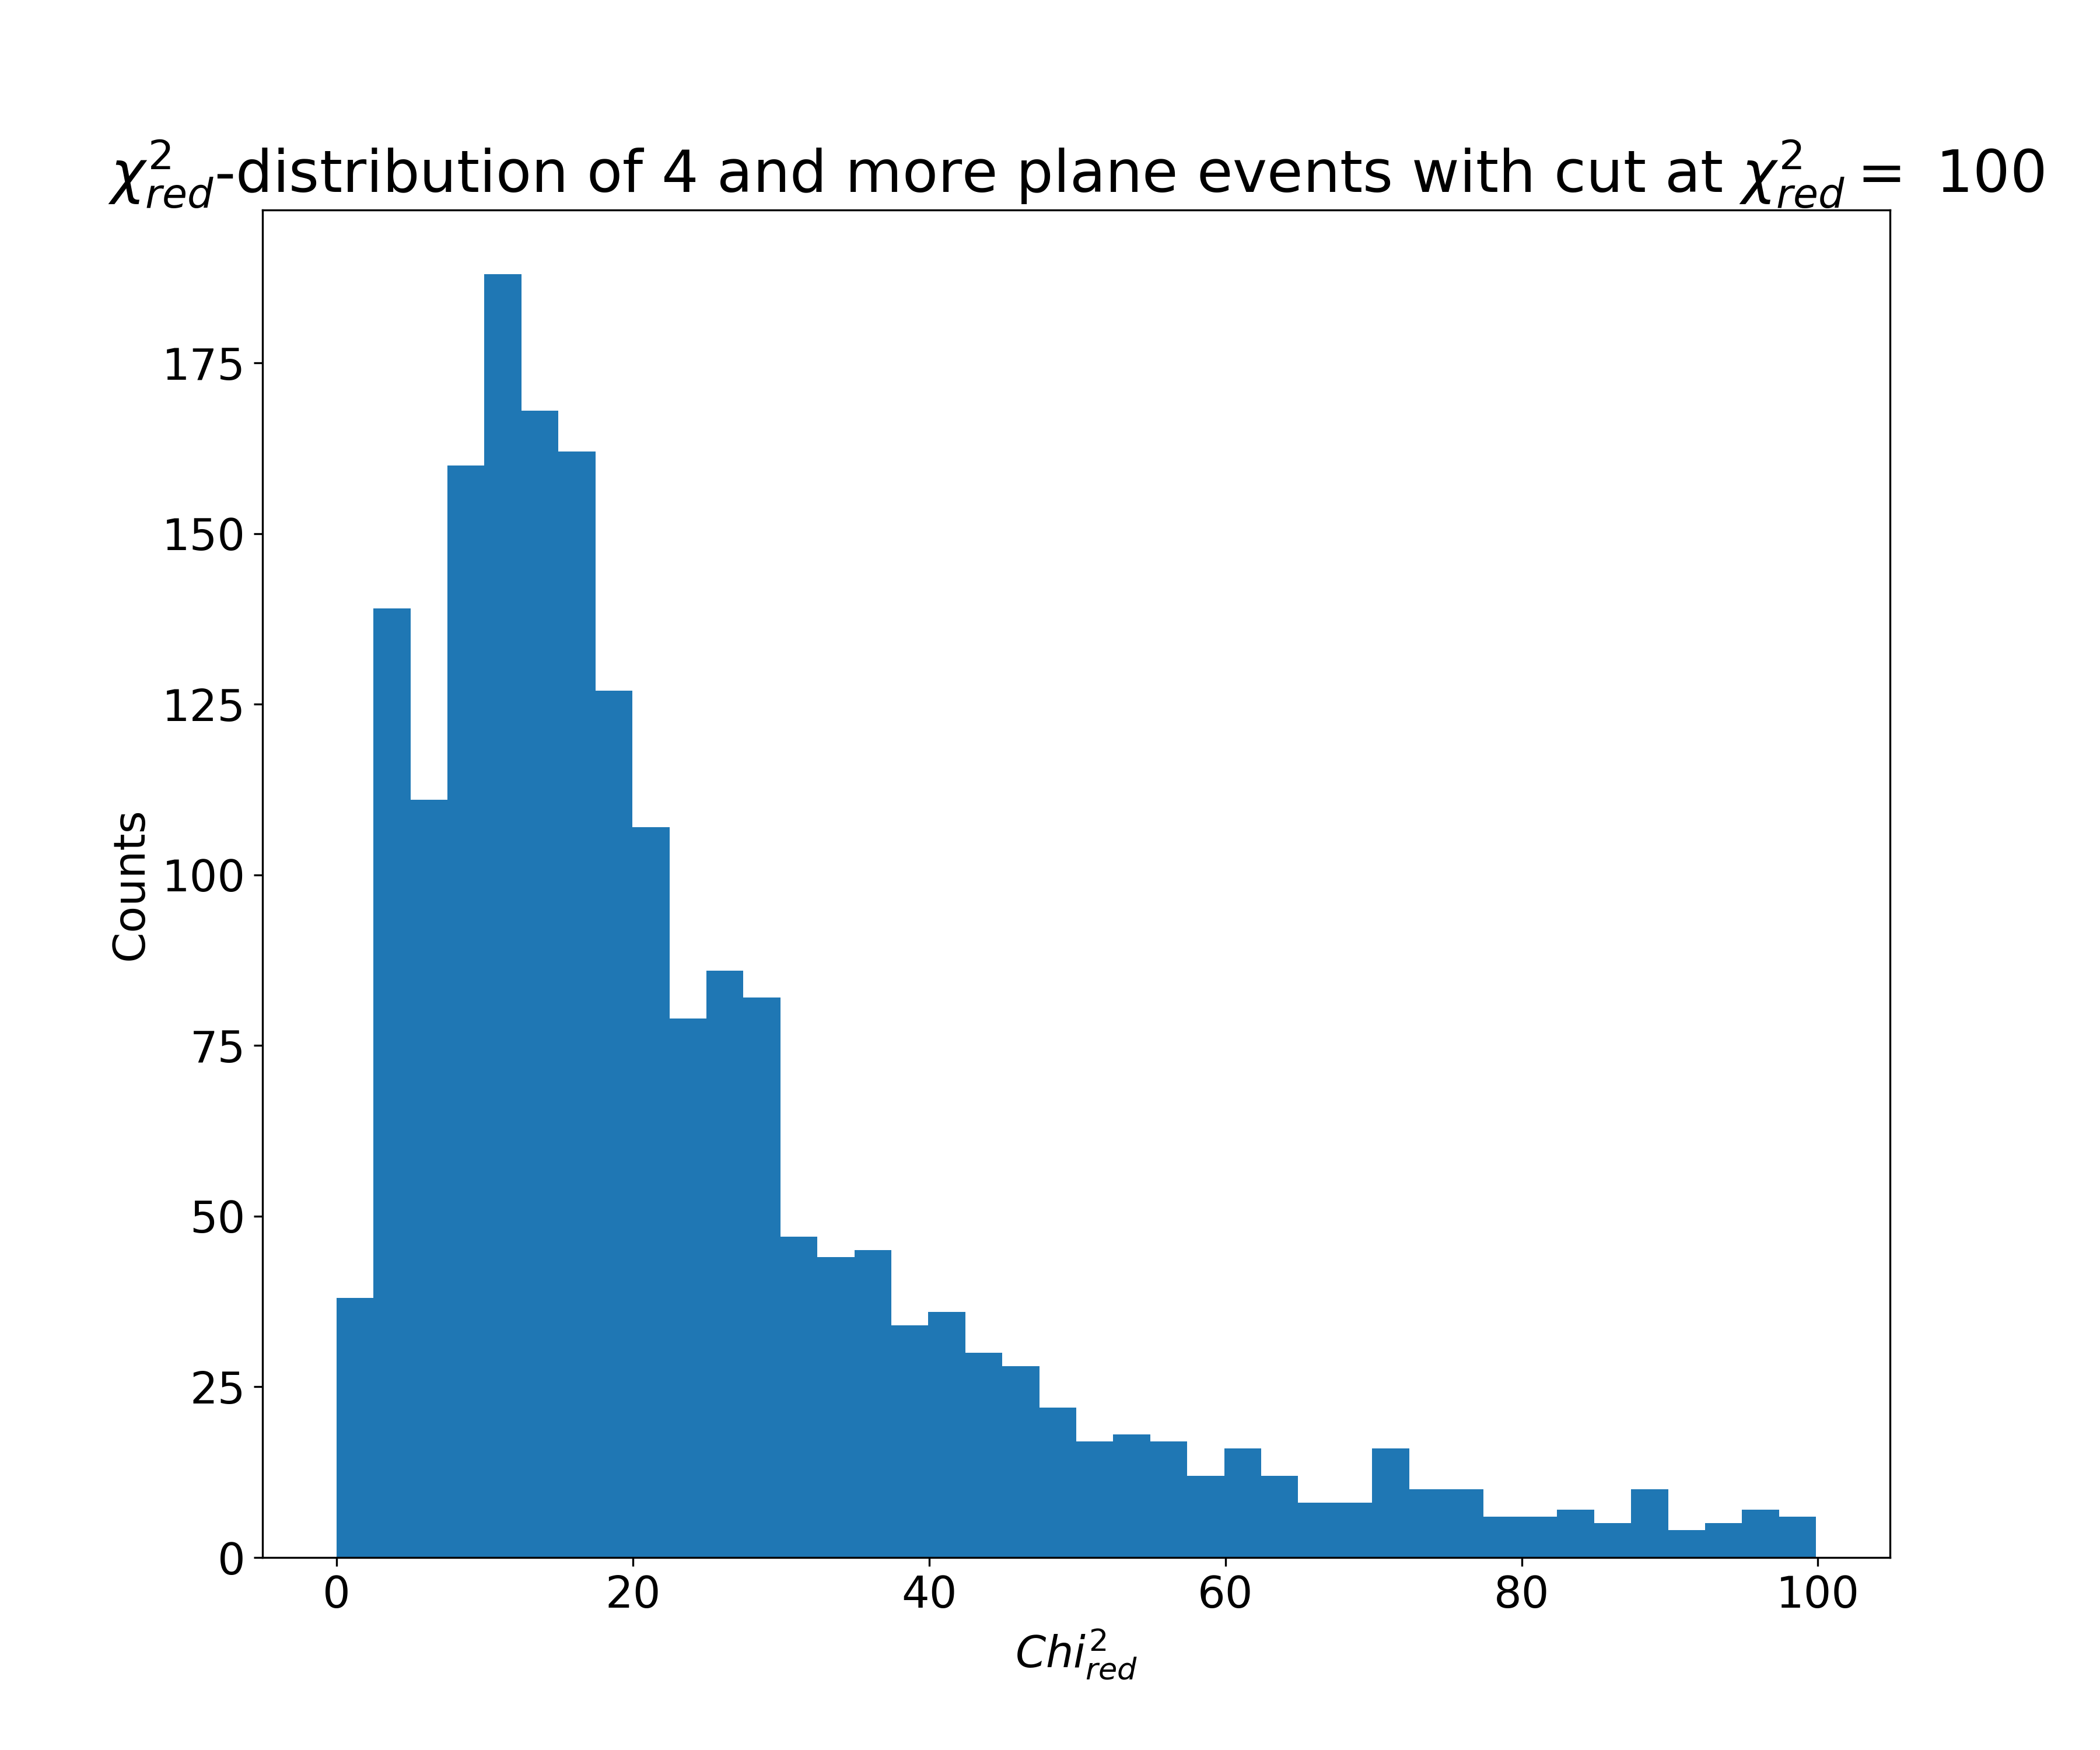
\includegraphics[width=.49\textwidth]{track_chi}
    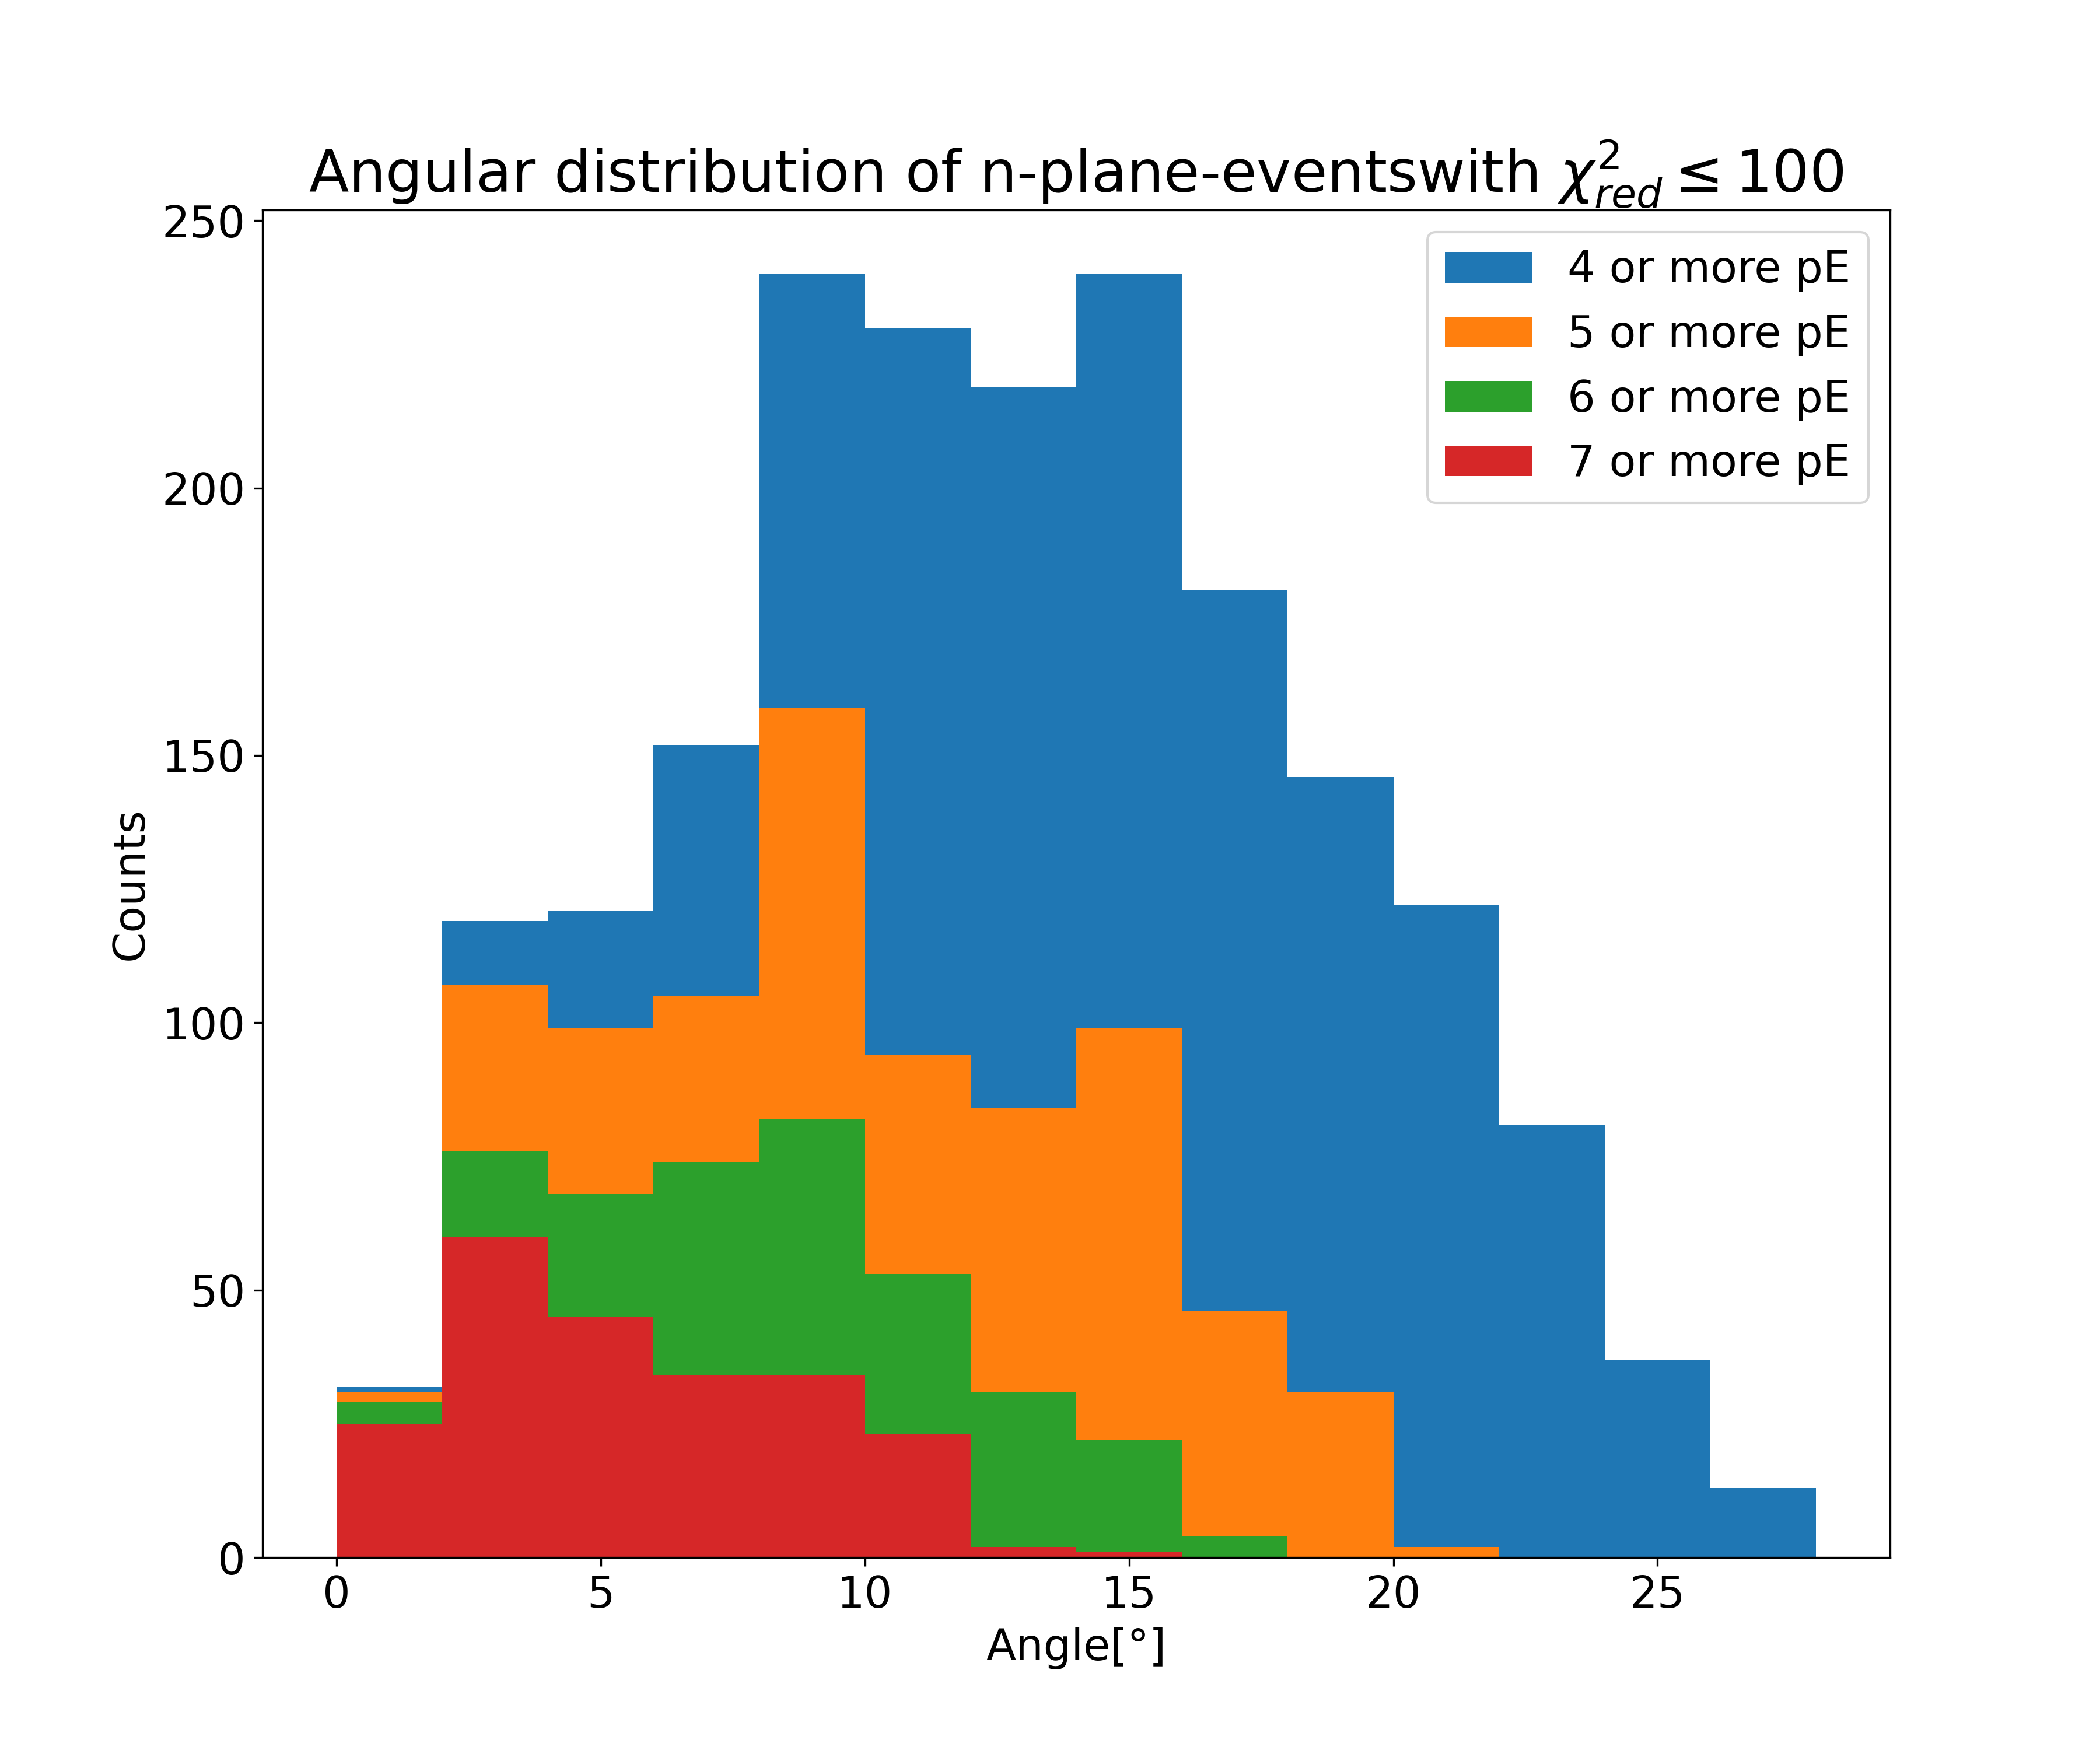
\includegraphics[width=.49\textwidth]{track_angle}
  \end{figure}
\end{frame}

%\begin{frame}{APENDIX}
%  \LARGE Muon rate calculation \normalsize \\[.5cm]
%\end{frame}

